\begin{center}
    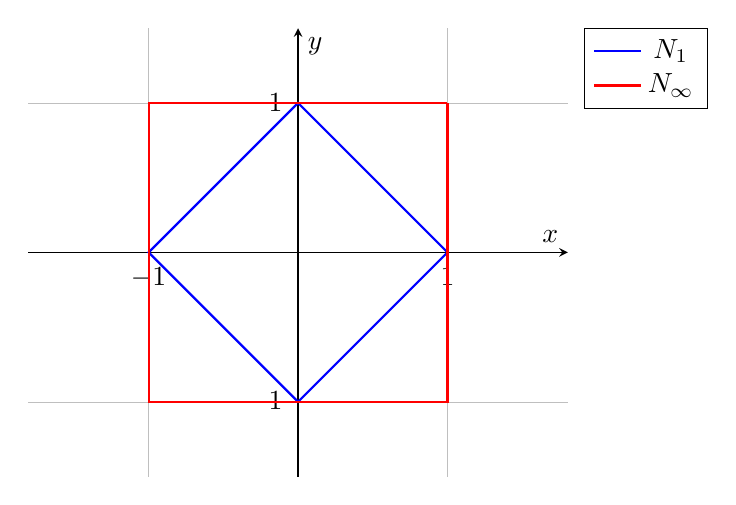
\begin{tikzpicture}
    \begin{axis}[
    axis equal,
    axis lines = middle,
    xmin = -1.5, xmax = 1.5,
    ymin = -1.5, ymax = 1.5,
    xlabel = {$x$},
    ylabel = {$y$},
    xtick = {-1, 0, 1},
    ytick = {-1, 0, 1},
    grid = both,
    major grid style = {line width=.2pt,draw=gray!50},
    minor grid style = {line width=.1pt,draw=gray!20},
    legend pos = outer north east,
    ]
    % Norme 1 (losange)
    \addplot[
    color=blue,
    mark=none,
    thick,
    ] coordinates {
    (1, 0) (0, 1) (-1, 0) (0, -1) (1, 0)
    };
    \addlegendentry{$N_1$}

    % Norme infinie (carré)
    \addplot[
    color=red,
    mark=none,
    thick,
    ] coordinates {
    (1, 1) (-1, 1) (-1, -1) (1, -1) (1, 1)
    };
    \addlegendentry{$N_\infty$}
    \end{axis}
    \end{tikzpicture}
\end{center}